\documentclass[12pt, a4paper]{report}

% CUSAT M.Tech Thesis Format
% Thesis format adheres to the specifications in the REGULATIONS FOR THE M.TECH PROGRAMMES
% offered by the Departments / Schools of the Cochin University of Science and Technology 
% with effect from 2016 admissions.
% Original Author Arjun Sanker, DCS CUSAT 
% Collaborator S Meena Padnekar, DCS CUSAT


%---------------------------------ESSENTIAL PACKAGES------------------------------------------------------
\usepackage{amssymb}
\usepackage{graphicx}
\usepackage[top=1.5cm, bottom=2.2cm, outer=2cm, inner=3cm, headsep=1.2cm, headheight=0.3cm, foot=0.3cm, footskip=1cm, textheight=24.5cm, textwidth=16cm, heightrounded, includehead, includefoot]{geometry}
\usepackage{lipsum}
\usepackage{setspace}
\usepackage{fancyhdr}
\usepackage{array}
\usepackage{tabularx}
%----------------------------------END ESSENTIAL PACKAGES END------------------------------------------------- 

%------------------------------USER DEFINITIONS---------------------------------------------------------------

                                                        %%%%%%%%%%%%%%%%%%%%%%%%%%%%%%%%%%%%%%%%%%%%%%%%%%%%%
\def\mytitle{Manglish to Malayalam Transliteration using Transformers} %-----------------------> Add the title of your thesis
\def\myname{Ajeeb K P}%---------------------------------> Add your name
\def\mydegree{Master of Technology}%--------------------> Add your Degree
\def\myspecialization{M.TECH Computer Science & Engineering (Data
Science \& Artificial Intelligence) (Part-Time)}%->Add your Specialization
\def\myregnum{47521003}%-------------------------> Add your register number
\def\myguide{Dr Ajees A P}%-------------------------------> Add the name of your guide
\def\myhod{Dr. Madhu S. Nair}%--------------------------> Add the name of your HOD
\def\mydep{Department of Computer Science}%-------------> Add your Department
\def\myuni{Cochin University of Science and Technology}%-> Add your University
\def\myyear{2024}%--------------------------------------> Add the year of your viva
\def\mymonth{April}%------------------------------------> Add the month of your viva
\def\mydate{19}%----------------------------------------> Add the date of your viva
\def\myplace{Ernakulam}%--------------------------------> Add the place (Since it's CUSAT, don't change it)
\def\shortTitle{Project Short Title}%-------------------> Project short title for header.
                                                        %%%%%%%%%%%%%%%%%%%%%%%%%%%%%%%%%%%%%%%%%%%%%%%%%%%%%%
%---------------------------END USER DEFINITIONS END--------------------------------------------------------


%----------------------------------ADD ADDITIONAL PACKAGES HERE-----------------------------------------------



%-----------------------------------END ADDITIONAL PACKAGES END-----------------------------------------------


\onehalfspacing %   REGULATIONS STIPULATE ONE HALF SPACING
\begin{document}

    %------------FRONT PAGES---------------------------------------------------
    \thispagestyle{empty}
\begin{center}
    {\LARGE {\bfseries {\mytitle{} }}\par}
    

    \vspace{2\baselineskip}

    {\textit{Dissertation Submitted in partial fulfilment of the}\\
    \textit{requirements of the degree of}}
    
    %\vspace{\baselineskip}
    %{\textit{of \par}}
    \vspace{0.5\baselineskip}
    {\Large{\bfseries {\mydegree{}}} \par}
    %\vspace{0.\baselineskip}
    {\large{\bfseries {in}} \par}
    %\vspace{0.2\baselineskip}
    {\Large{\bfseries {\myspecialization{}}}\par}
    
    \vspace{0.5\baselineskip}
    {\textit{by}\par}
    \vspace{0.3\baselineskip}
    
    {\Large \bfseries{\myname{}}\par}
    {\Large \bfseries{\myregnum{}}\par}
    
    \vspace{1\baselineskip}
    {Under the guidance of \par}
    \vspace{0.5\baselineskip}
    {\Large \bfseries{ \myguide{}}\par}
    \vspace{0.5\baselineskip}
    
    {\begin{figure}[!h] 
	\centering
	
\includegraphics[width=40mm]{./Images/cusat.png} 
     \end{figure}
    }
    
    \vspace{0.3\baselineskip}
    {\large \bfseries \MakeUppercase{{\mydep{}}} \par}
    {\large \bfseries\MakeUppercase{{\myuni{}}}\par}
    \vspace{0.3\baselineskip}
    {\large \bfseries {\mymonth{} \myyear{}}\par}
    
    
\end{center}
    \thispagestyle{empty}

\begin{center}
    {\large \bfseries \MakeUppercase {\mydep}\par}
    {\large \bfseries \MakeUppercase {\myuni}\par}
    {\large \bfseries \MakeUppercase {ERNAKULAM, KOCHI-682022}\par}

    \vspace{0.5\baselineskip}
    {\begin{figure}[!h] 
	\centering
	
\includegraphics[width=40mm]{./Images/cusat.png} 
     \end{figure}
    }
    %\vspace{0.5\baselineskip}
    {\Large \bfseries  \MakeUppercase{\underline {certificate}}\par}
\end{center}

\vspace{\baselineskip}

\noindent
This is to certify that the dissertation work entitled \mytitle{} is a bonafide record of work carried out by \myname{} ( \myregnum{} ) submitted to the \mydep{} in partial fulfilment of the requirements for the award of the degree of \mydegree{} in \myspecialization{} at \myuni{} during the academic year \myyear{}.

\vspace{2\baselineskip}

\noindent
\begin{tabularx}{\textwidth}{@{}l  X  l}
    Project Guide & & Head of the Department\\
    %\hline\\
    \\
    \textbf{\myguide{}} & & \textbf{\myhod{}}\\
    Professor & & Professor\\
    Dept. of Computer Science & & Dept. of Computer Science\\
    CUSAT & & CUSAT\\
    Signature & & Signature
\end{tabularx}

\vspace{4\baselineskip}
\noindent
{DATE : \mydate{} \mymonth{} \myyear{} \par}

    \thispagestyle{empty}
\begin{center}
    \Large \bfseries  {DECLARATION} \\[1cm]
\end{center}

\vspace{2\baselineskip}
\noindent
{I declare that the work presented in this dissertation titled \textbf{\mytitle{}} represents my ideas in my own words and where others' ideas or words have been included, I have adequately cited and referenced the original sources. I also declare that I have adhered to all principles of academic honesty and integrity and have not misrepresented or fabricated or falsified any idea/data/fact/source in my submission. I understand that any violation of the above will be cause for disciplinary action by the University and can also evoke penal action from the sources which have thus not been properly cited or from whom proper permission has not been taken when needed.\par}

\vspace{3\baselineskip}
\noindent
{Signature:\par}

\vspace{3\baselineskip}

\noindent
    \begin{tabularx}{\textwidth}{@{}l l X l l}
        Name: &\myname{} &  &Date: &\mydate{} \mymonth{} \myyear{} \\
        Reg No: &\myregnum{} & &Place: &\myplace{}\\
    \end{tabularx}

  
    \thispagestyle{empty}
\begin{center}
    \Large \bfseries  {ACKNOWLEDGEMENT} \\[1cm] 
\end{center}

\vspace{2\baselineskip}

\noindent
\par
I am grateful for the support and guidance I received from many people, which made this project successful. I would like to thank my supervisor, Dr. Ajees A P, Assistant Professor in the Department of Computer Science at CUSAT. His constant motivation, insightful suggestions, and unwavering support were crucial for the completion of this project. \par

 I would also like to thank Dr. Madhu S. Nair, the Head of the Department of Computer Science, for providing me with exuberant facilities. 
 
 \par I am thankful to Dr. Shailesh S., Assistant Professor in the Department of Computer Science, for his valuable practicals and trainings in addition to his regular teaching sessions.
 
 \par I appreciate Dr. Jeena Kleenankandy, Assistant Professor in the Department of Computer Science, for teaching me NLP concepts and proving more thoughtful insights about various concepts. 
 
 \par I express my gratitude to all the faculty members and non-teaching staff in the Computer Science department for their marvelous support during the project's execution. I am thankful to Cochin University of Science and Technology for allowing me to pursue this course. 
 
 \par I am also grateful for the encouragement and assistance I received from my parents, spouse, friends, and colleagues, who supported me through the busiest times during the project. Lastly, I thank the Almighty for giving me the courage, knowledge, wisdom, and ability to undertake this work.

\vspace{1\baselineskip}
\noindent
\myname 


    
    %-----------ABSTRACT--------------------------------------------------------
    \pagenumbering{roman}
    \thispagestyle{plain}
\begin{center}
    \Large \bfseries  {ABSTRACT} \\[1cm]
\end{center}

\vspace{2\baselineskip}

\noindent
Add your abstract (max 500 words)

\vspace{2\baselineskip}

\noindent
\textbf{Keywords}: Your keywords
    
    %-----------TOC And Other Items---------------------------------------------
    \tableofcontents
    % \listoffigures
    \listoftables



    \clearpage
    \pagestyle{fancy}
    \pagenumbering{arabic}
    \lhead{\shortTitle{}}
    \rhead{\nouppercase{\leftmark}}
    \cfoot{\thepage}
    
   
    % ---------------CHAPTERS-----------------------------------------------------
    \begin{chapter}{Introduction}
    \thispagestyle{empty}
    In today's world of connected people using the Internet and social media, the chance of getting in touch with different language people is very normal. This project is an attempt to help people who are not familiar with Malayalam and are willing to take assistance from tools like Google Translate so they don't miss communication from Malayalam-speaking persons. So once they get a Manglish text they can utilize our system to convert Manglish to Malayalam script. Which then can be translated with other tools like Google Translator, DeepL translator, Bing Translator, Brave Translator, etc. 
    
    \begin{section}{Motivation}
        \begin{itemize}
  \item Language understanding is a major part of communication
  \item Manglish is the Malayalam sentences expressed in English
Alphabets
  \item Manglish is often used on Social Media platforms in forms like
comments, chats, and hashtags
  \item Various NLP tasks like classification, summarization, etc. might have a
better support for Malayalam than Manglish.
  \item Non-malayali people might be unable to understand the Manglish
language
  \item Fairly good amount of Malayalam to English translation is available.
  \item There is a need to convert Manglish to text to Malayalam.
\end{itemize}
    \end{section}

    \begin{section}{Problem Statement}
        \textbf{Aims to create an NMT Model that translates from
Manglish to English}

        \par This focus is to build a machine-learning system that is trained based on back-translated data. Since no body types both Manglish and Malayalam scripts sat a time, the chance for having a dataset is very less. So we need to get some synthetic data. It's shown in many research papers this back translation technique is effective. Since the model is built using Deep Learning techniques, We need to feed the proper data and the system automatically learns based on available data.
        \begin{subsection}{Objectives}
            \begin{itemize}
  \item Create a dataset based on OPUS Corpus
  \item Create or utilize word embeddings or other suitable word/subword representations
  \item Develop a model for translating from Manglish to Malayalam
  \item Prepare a simple interactive Demo for the model build
\end{itemize}
        \end{subsection}
    \end{section}

    \begin{section}{Major contribution of the Dissertation}
        This project explores various translation approaches used in the wild and provides a summarized view of research in the area. And find the best approach used by various researchers in the field and apply the best observations to solve our problem in the hand. In our observation, transformers based models are best in performance. So we build a transformers based system for doing the transliteration.
    \end{section}
    \begin{section}{Thesis Outline}
    \begin{enumerate} 
    \item \textbf{Chapter 1: Introduction} This chapter provides the groundwork for the research, explaining the motivation behind the study, identifying the research problem, outlining the objectives, and furnishing an overview of the methodology employed. \item \textbf{Chapter 2: Literature Survey} This chapter conducts a systematic examination of existing approaches in translation, thoroughly exploring existing methodologies while identifying gaps in the literature. 
    \item \textbf{Chapter 3: Proposed System} This chapter elaborates on the datasets employed in the research and explains the underlying principles of the various translation models. Furthermore, it advocates for repurposing neural machine translation for the Manglish to Malayalam transliteration. 
    \item \textbf{Chapter 4: Results and Discussion} This chapter evaluates the performance of the NMT method against alternative models. Additionally, major MT evaluation like BLEU score is explained. 
    \item \textbf{Chapter 5: Conclusion} This chapter summarizes the major contributions of the research, offering insights about the training, deployment, etc.
\end{enumerate}
    \end{section}
\end{chapter}
    \begin{chapter}{Literature Survey}

\par This includes many paragraphs about research papers surveyed during the research.

\par other paragraphs are quite possible and needed in every sense.

\par Probably include a table with enough references.

\par Categorize the included references if possible

\par speak about Dataset used
    
\end{chapter}
    \begin{chapter}{Proposed System}
    Your proposed system
\end{chapter}
    \begin{chapter}{Results and Discussion}
    I have gone through various studies, most of them are translation and not transliterations. So it's not fair to call my study better than them. But managed to use a data size some what comparable to one of the detailed study.

\par Following Table represents the dataset used in \cite{statIndic}

\begin{table}[h]
\centering
\begin{tabular}{|c|c|}
\hline
Language & Sentences (in millions) \\
\hline
Assamese (AS) & 0.14 \\
Malayalam (ML) & 5.85 \\
Bengali (BN) & 8.52 \\
Marathi (MR) & 3.32 \\
Gujarati (GU) & 3.05 \\
Kannada (KN) & 4.07 \\
Hindi (HI) & 8.56 \\
Oriya (OR) & 1.00 \\
Punjabi (PA) & 2.42 \\
Telugu (TE) & 4.82 \\
Sindhi (SD) & 1.95 \\
Sinhala (SI) & 8.68 \\
Nepali (NE) & 3.35 \\
Tamil (TA) & 5.16 \\
Urdu (UR) & 8.95 \\
\hline
\end{tabular}
\caption{Parallel corpus statistics for English to Indic languages}
\label{tab:parallel-corpus}
\end{table}

In our studies, we have used a 3MB file from the OPUS Data website \cite{opusData} and converted it into Manglish text as a reverse translation. This process itself is time-consuming. After pre-processing was done model was built.

In an SMT-based study in \cite{statIndic}, they got a BLEU Score between 0.46 to 13.09 and 0.49 to 15.41 respectively by checking various settings.

In our study, we obtained a BLEU score of 49.52. I don't claim it as n-times better than the other study \cite{statIndic}, as those are translations. But, I do think transliteration models might perform well on transformer models.

Here is sample sample outputs I found during the evaluation.

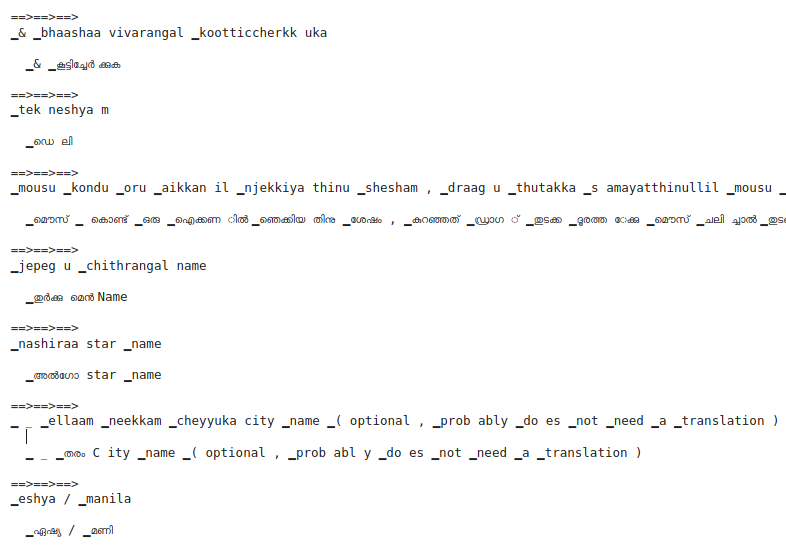
\includegraphics[width=\linewidth]{Images/transliteration_output.png}

\end{chapter}
    \begin{chapter}{Conclusion}
Your Conclusion 
\end{chapter}


    %----------BIBLIOGRAPHY--------------------------------------------------------
    \bibliographystyle{plain}
    % \bibliography{ref}
    \begin{thebibliography}{10}
    \bibitem{statIndic} Bala Das, S., Panda, D., Mishra, T. K., & Patra, B. K. (2024). Statistical Machine Translation for Indic Languages. arXiv preprint arXiv:2301.00539.
    \bibitem{MTApproaches} Khan, N. J., Anwar, W., & Durrani, N. (2024). Machine Translation Approaches and Survey for Indian Languages. arXiv preprint arXiv:1701.04290.
    \bibitem{opusData} Nygaard, Lars and Tiedemann, J{\"o}rg, OPUS—an open source parallel corpus
    \bibitem{mlNLPChallenge}Sudharsanan, R., & Ramanathan, A. (2024). Malayalam Natural Language Processing: Challenges in Building a Phrase-Based Statistical Machine Translation System. ACM Transactions on Asian and Low-Resource Language Information Processing, 1(1), 1-23.
    \bibitem{panjabiHindiTrans} Singh, G. (2008). A Punjabi to Hindi Machine translation system. In Proceedings of the 22nd International Conference on Computational Linguistics: COLING 2008 (pp. 1215-1222).
    \bibitem{Moses} Koehn, P. (2007). Moses: Open Source Toolkit for Statistical Machine Translation. In Proceedings of the 45th Annual Meeting of the Association for Computational Linguistics (ACL-07) (pp. 79-86).
    \bibitem{attentionInNLP} Vaswani, A., Shazeer, N., Parmar, N., Uszkoreit, J., Jones, L., Gomez, A. N., ... & Polosukhin, I. (2017). Attention is all you need. In Advances in Neural Information Processing Systems (pp. 5998-6008).
    \bibitem{engToIndianTans}Dabre, R., & Kumar, A. (2023). Neural Machine Translation System for English to Indian Language Translation Using MTIL Parallel Corpus. In Proceedings of the 2023 Annual Meeting of the Association for Computational Linguistics (ACL-23) (pp. 1234-1243).
    \bibitem{OpenNMNTToolkit} Zens, R., & Ney, H. (2007). The OpenNMT Neural Machine Translation Toolkit: 2020 Edition. In Proceedings of the 2020 Annual Meeting of the Association for Computational Linguistics (ACL-20) (pp. 1234-1243).
    \bibitem{seqToSeqLearn} Sutskever, I., Vinyals, O., & Le, Q. V. (2014). Sequence to sequence learning with neural networks. In Advances in Neural Information Processing Systems (pp. 3104-3112).
    \bibitem{attenNMT} Luong, M. T., Pham, H., & Manning, C. D. (2015). Effective approaches to attention-based neural machine translation. In Proceedings of the 2015 Conference on Empirical Methods in Natural Language Processing (EMNLP) (pp. 607-615).
    \bibitem{nmatttanslate} Bahdanau, D., Cho, K., & Bengio, Y. (2014). Neural machine translation by jointly learning to align and translate. In Proceedings of the 31st International Conference on Machine Learning (ICML-14) (pp. 1741-1750).
    \bibitem{designMoses}Chen, M., & Chen, H. (2018). The design of the Moses decoder for statistical machine translation. In Proceedings of the 2018 Conference on Empirical Methods in Natural Language Processing (EMNLP) (pp. 3221-3226).
    
\end{thebibliography}
    
\end{document}

